\documentclass[12pt,a4paper]{article}
\usepackage[utf8]{inputenc}
\usepackage[T1]{fontenc}
\usepackage[spanish]{babel}
\usepackage{geometry}
\usepackage{graphicx}
\usepackage{float}
\usepackage{hyperref}
\usepackage{listings}
\usepackage{xcolor}
\usepackage{booktabs}
\usepackage{array}
\usepackage{caption}
\usepackage{subcaption}
\usepackage{amsmath}
\usepackage{titlesec}
\usepackage{fancyhdr}
\usepackage{mdframed}
\usepackage{enumitem}

\geometry{
  top=2.5cm,
  bottom=2.5cm,
  left=3cm,
  right=3cm
}

% Colores
\definecolor{codebg}{RGB}{13,17,23}
\definecolor{codetext}{RGB}{201,209,217}
\definecolor{accent}{RGB}{88,166,255}
\definecolor{green}{RGB}{63,185,80}
\definecolor{orange}{RGB}{210,153,34}
\definecolor{red}{RGB}{248,81,73}
\definecolor{gray}{RGB}{110,118,129}

% Configuración de listings
\lstset{
  backgroundcolor=\color{codebg},
  basicstyle=\ttfamily\footnotesize\color{codetext},
  keywordstyle=\color{accent}\bfseries,
  stringstyle=\color{green},
  commentstyle=\color{gray}\itshape,
  numbers=left,
  numberstyle=\tiny\color{gray},
  stepnumber=1,
  numbersep=8pt,
  frame=single,
  framerule=0.5pt,
  rulecolor=\color{gray},
  breaklines=true,
  breakatwhitespace=false,
  showstringspaces=false,
  tabsize=4,
  captionpos=b
}

% Encabezado y pie de página
\pagestyle{fancy}
\fancyhf{}
\rhead{MMU Simulator}
\lhead{Informe Técnico}
\rfoot{\thepage}
\lfoot{2026}

% Título personalizado
\hypersetup{
  colorlinks=true,
  linkcolor=accent,
  urlcolor=accent,
  citecolor=accent
}

% ─────────────────────────────────────────────
\begin{document}

% ─── PORTADA ──────────────────────────────────
\begin{titlepage}
  \centering
  \vspace*{2cm}

  {\Huge\bfseries Simulador de Unidad de Gestión\\[0.3em]
  de Memoria (MMU)\par}

  \vspace{0.5cm}
  {\large\color{gray} Informe Técnico del Proyecto\par}

  \vspace{2cm}

  \begin{mdframed}[linecolor=accent,linewidth=1.5pt,leftmargin=2cm,rightmargin=2cm]
    \centering\vspace{0.3cm}
    {\normalsize Simulador educativo de una \textbf{MMU (Memory Management Unit)} que
    demuestra en tiempo real cómo juegos y aplicaciones pesadas compiten
    por los marcos de RAM, con visualización interactiva de PTBR, TLB,
    tabla de páginas y el algoritmo Óptimo de Belady.}
    \vspace{0.3cm}
  \end{mdframed}

  \vspace{2cm}

  \begin{tabular}{ll}
    \textbf{Lenguaje:}    & Python 3.8+ \\[4pt]
    \textbf{Framework:}   & Flask 3.0+ \\[4pt]
    \textbf{Memoria real:}& \texttt{ctypes} (buffers del SO) \\[4pt]
    \textbf{Despliegue:}  & Render (Gunicorn) \\[4pt]
    \textbf{Repositorio:} & GitHub \\[4pt]
    \textbf{Fecha:}       & Marzo 2026 \\
  \end{tabular}

  \vfill
  {\small Documento generado a partir del historial de desarrollo del proyecto}
\end{titlepage}

% ─── TABLA DE CONTENIDOS ──────────────────────
\tableofcontents
\newpage

% ─── 1. INTRODUCCIÓN ──────────────────────────
\section{Introducción}

La \textbf{Unidad de Gestión de Memoria} (MMU, \textit{Memory Management Unit}) es el componente
de hardware responsable de traducir direcciones de memoria virtuales a físicas. Es un concepto
fundamental en sistemas operativos modernos que permite la multiprogramación, el aislamiento entre
procesos y el uso eficiente de la RAM.

Este proyecto implementa un \textbf{simulador educativo completo} de una MMU, diseñado para
visualizar de manera interactiva y animada todos los mecanismos de gestión de memoria: paginación,
tabla de páginas, TLB, fallos de página y el algoritmo de reemplazo Óptimo de Belady.

\subsection{Motivación}

Los conceptos de paginación y gestión de memoria suelen ser abstractos y difíciles de visualizar
a partir de diagramas estáticos. Este simulador nació con la necesidad de:

\begin{itemize}[leftmargin=1.5cm]
  \item Hacer \textit{tangible} el comportamiento de la MMU con animaciones en tiempo real
  \item Usar procesos realistas (juegos, editores, motores 3D) en lugar de ejemplos artificiales
  \item Demostrar el algoritmo Óptimo con análisis de uso futuro visible al estudiante
  \item Permitir navegación paso a paso, incluyendo \textit{retroceso} para examinar transiciones
\end{itemize}

\subsection{Alcance}

El proyecto comprende dos versiones:
\begin{enumerate}[leftmargin=1.5cm]
  \item \textbf{Versión terminal} (\texttt{mmu\_simulador.py}): operación con RAM real via
        \texttt{ctypes}, salida ANSI, modo paso a paso o automático.
  \item \textbf{Versión web} (\texttt{mmu\_gui.py}): interfaz Flask con HTML/CSS/JS embebido,
        visualizaciones interactivas, animaciones y API REST.
\end{enumerate}

\newpage

% ─── 2. ARQUITECTURA ──────────────────────────
\section{Arquitectura del Sistema}

\subsection{Estructura de archivos}

\begin{lstlisting}[language=bash, caption=Estructura del proyecto]
s04/
├── mmu_simulador.py   # Simulador terminal (ctypes, TLB, Belady, ANSI)
├── mmu_gui.py         # App web Flask: simulacion + HTML/CSS/JS embebido
├── requirements.txt   # Flask, psutil, gunicorn
├── render.yaml        # Despliegue Render
├── DEPLOY.md          # Guia de despliegue
├── informe.tex        # Este informe
└── captures/
    ├── cap01.png      # Panel de procesos y uso de RAM
    ├── cap02.png      # PTBR apuntando a tabla de paginas
    ├── cap03.png      # Vista completa con PAGE FAULT
    ├── cap04.png      # Historial de eventos
    └── cap05.png      # TLB con slots coloreados
\end{lstlisting}

\subsection{Stack tecnológico}

\begin{table}[H]
\centering
\begin{tabular}{>{\bfseries}lll}
\toprule
Componente & Tecnología & Propósito \\
\midrule
Lenguaje & Python 3.8+ & Lógica completa del simulador \\
Memoria real & \texttt{ctypes} & Buffers de 4 KB asignados por el SO \\
I/O de disco & \texttt{tempfile}, \texttt{struct} & Simula swap/paginación en disco \\
Web framework & Flask 3.0+ & Servidor HTTP y API REST \\
Monitoreo & \texttt{psutil} 5.9+ & Detección de apps pesadas reales \\
Producción & Gunicorn 21.0+ & Servidor WSGI multi-worker \\
Despliegue & Render & PaaS con autodespliegue desde Git \\
Frontend & HTML/CSS/JS puro & Embebido en string Python \\
\bottomrule
\end{tabular}
\caption{Stack tecnológico del proyecto}
\end{table}

\subsection{Flujo de la API REST}

La versión web expone cinco endpoints:

\begin{table}[H]
\centering
\begin{tabular}{lll}
\toprule
\textbf{Método} & \textbf{Ruta} & \textbf{Acción} \\
\midrule
POST & \texttt{/api/inicializar} & Crea motor con N marcos, genera cadena de accesos \\
POST & \texttt{/api/avanzar}     & Avanza un paso (guarda snapshot antes) \\
POST & \texttt{/api/retroceder}  & Restaura el snapshot anterior \\
GET  & \texttt{/api/estado}      & Retorna estado completo (TLB, RAM, stats, etc.) \\
POST & \texttt{/api/reset}       & Reinicia la simulación \\
\bottomrule
\end{tabular}
\caption{Endpoints de la API REST}
\end{table}

\newpage

% ─── 3. SIMULACIÓN DE PROCESOS ────────────────
\section{Simulación de Procesos Realistas}

\subsection{Detección de aplicaciones pesadas}

El simulador usa \texttt{psutil} para inspeccionar los procesos en ejecución del sistema
operativo. Si detecta aplicaciones pesadas conocidas (juegos, editores de imagen, motores
3D, herramientas de streaming), las usa como base para la simulación:

\begin{lstlisting}[language=python, caption=Detección de apps pesadas con psutil]
_APPS_PESADAS = {
    "minecraft", "unity", "unreal", "blender",
    "photoshop", "premiere", "aftereffects",
    "obs", "streamlabs", "discord",
    "steam", "epicgames", "godot",
}

def _detectar_procesos():
    procs = []
    tiene_app_pesada = False
    for p in psutil.process_iter(["name","memory_info","pid"]):
        nombre_lower = p.info["name"].lower()
        if any(k in nombre_lower for k in _APPS_PESADAS):
            tiene_app_pesada = True
            procs.append(...)

    if not tiene_app_pesada:
        # Fallback: perfiles predefinidos de apps pesadas
        procs = FALLBACK_PROCS
    return procs
\end{lstlisting}

\subsection{Perfiles predefinidos (fallback)}

Cuando no se encuentran aplicaciones pesadas en el sistema (por ejemplo, en un servidor
de producción sin GUI), se usan perfiles predefinidos con valores de RAM realistas:

\begin{table}[H]
\centering
\begin{tabular}{llll}
\toprule
\textbf{App} & \textbf{Ícono} & \textbf{RAM simulada} & \textbf{Páginas} \\
\midrule
Minecraft     & ⛏️  & 2.0 GB & proporcional \\
Photoshop     & 🎨  & 1.8 GB & proporcional \\
Blender       & 🔶  & 1.4 GB & proporcional \\
Unity Editor  & 🕹️  & 1.1 GB & proporcional \\
OBS Studio    & 🎥  & 600 MB & proporcional \\
Discord       & 🎙️  & 300 MB & proporcional \\
\bottomrule
\end{tabular}
\caption{Perfiles predefinidos de aplicaciones simuladas}
\end{table}

\subsection{Descripciones de acceso por tipo de app}

La función \texttt{\_desc\_acceso()} genera descripciones semánticas según el tipo de
aplicación, haciendo la simulación más comprensible:

\begin{itemize}[leftmargin=1.5cm]
  \item \textbf{Juegos (Minecraft):} ``Texturas 4K chunk \#42'', ``Física Rigidbody pool'', ``Audio engine buffer''
  \item \textbf{Editores de imagen (Photoshop):} ``Buffer capa Curves adj.'', ``Exportar RAW 48-bit'', ``LUT de color 3D''
  \item \textbf{3D/Render (Blender):} ``Malla 3D subdiv. lvl4'', ``Path tracing tile (32×32)'', ``BVH traversal buffer''
  \item \textbf{Motores (Unity):} ``Compilación JIT script'', ``Asset bundle streamed'', ``Shaders HLSL compilados''
  \item \textbf{Streaming (OBS):} ``Encoding H.264 GOP'', ``Captura frame display'', ``Audio mix 7.1''
\end{itemize}

\begin{figure}[H]
  \centering
  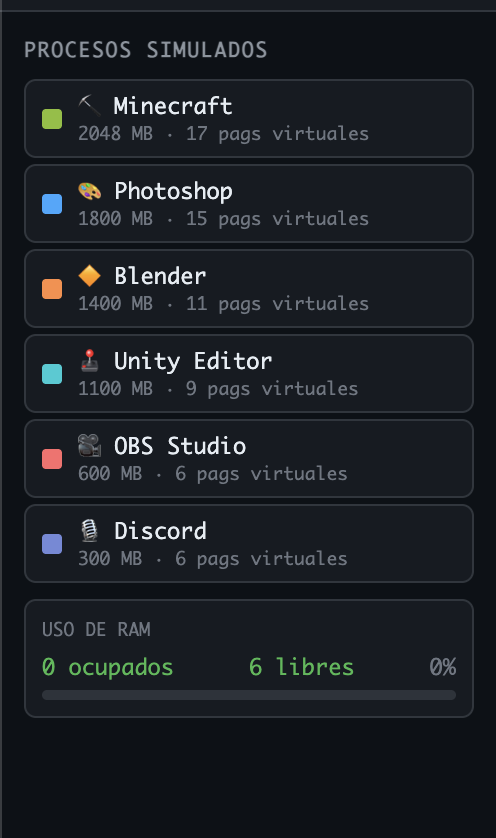
\includegraphics[width=0.85\textwidth]{captures/cap01.png}
  \caption{Panel izquierdo: lista de procesos simulados con barras de uso de RAM proporcionales al consumo real de cada aplicación. Cada proceso tiene un color único y un ícono representativo.}
\end{figure}

\newpage

% ─── 4. CONCEPTOS DE MMU IMPLEMENTADOS ────────
\section{Conceptos de MMU Implementados}

\subsection{Paginación con memoria real}

La implementación usa \texttt{ctypes} para asignar buffers de 4 KB directamente en el
espacio de direcciones del proceso del sistema operativo:

\begin{lstlisting}[language=python, caption=Asignación de marcos físicos con ctypes]
class Marco:
    TAMANO = 4096  # 4 KB — tamano real de pagina del SO

    def __init__(self, id_marco: int):
        self.id = id_marco
        self.libre = True
        self._buf = (ctypes.c_uint8 * Marco.TAMANO)()
        self.dir_fisica = ctypes.addressof(self._buf)
        self.proceso = None
        self.pagina = None
        self.bits = {"P": 0, "D": 0, "R": 0}
\end{lstlisting}

Las direcciones reportadas en la interfaz son \textbf{direcciones físicas reales} del proceso
del sistema operativo, no simuladas.

\subsection{Tabla de páginas con bits P/D/R}

Cada proceso mantiene su propia tabla de páginas. Cada entrada contiene:

\begin{table}[H]
\centering
\begin{tabular}{>{\bfseries}cll}
\toprule
Bit & Nombre & Significado \\
\midrule
P & Presente  & La página está cargada en RAM (1) o en disco (0) \\
D & Dirty     & La página fue modificada y debe escribirse al disco antes de desalojar \\
R & Referenciado & La página fue accedida recientemente \\
\bottomrule
\end{tabular}
\caption{Bits de estado en la tabla de páginas}
\end{table}

\subsection{Registro PTBR}

El \textbf{PTBR} (\textit{Page Table Base Register}) es un registro del procesador que
apunta a la tabla de páginas del proceso actualmente en ejecución. La interfaz visualiza:

\begin{itemize}[leftmargin=1.5cm]
  \item El proceso actual con su ícono y color
  \item Una flecha que apunta hacia su tabla de páginas
  \item Todas las entradas de la tabla (en RAM o en disco)
  \item La entrada actualmente referenciada resaltada en azul con scroll automático
\end{itemize}

\begin{figure}[H]
  \centering
  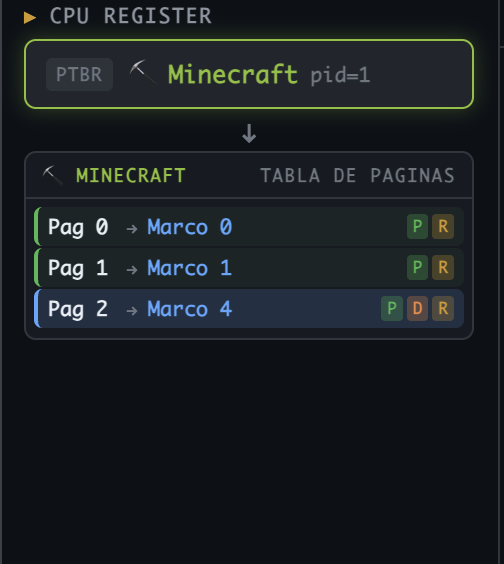
\includegraphics[width=0.85\textwidth]{captures/cap02.png}
  \caption{Panel izquierdo mostrando el registro PTBR de Minecraft (⛏️) apuntando a su tabla de páginas. La entrada resaltada en azul corresponde al acceso actual. Las entradas muestran el marco asignado o el estado ``disco''.}
\end{figure}

\newpage

\subsection{TLB — Translation Lookaside Buffer}

La TLB es una caché de traducciones de dirección virtual → física. El simulador implementa:

\begin{itemize}[leftmargin=1.5cm]
  \item \textbf{8 slots} de TLB con política de reemplazo FIFO
  \item \textbf{TLB Hit}: la traducción se encuentra en la TLB → acceso rápido sin consultar tabla de páginas
  \item \textbf{TLB Miss}: la traducción no está → consulta tabla de páginas, puede causar fallo de página
  \item Estadísticas en tiempo real de hit rate
\end{itemize}

La visualización muestra cada slot como una tarjeta con:
\begin{itemize}[leftmargin=1.5cm]
  \item Borde izquierdo del color de la aplicación dueña de la entrada
  \item Punto verde (válido) o rojo (inválido)
  \item Animación \texttt{glow-hit} cuando ocurre un TLB hit
  \item Animación \texttt{slide-in} al agregar una nueva entrada
\end{itemize}

\begin{figure}[H]
  \centering
  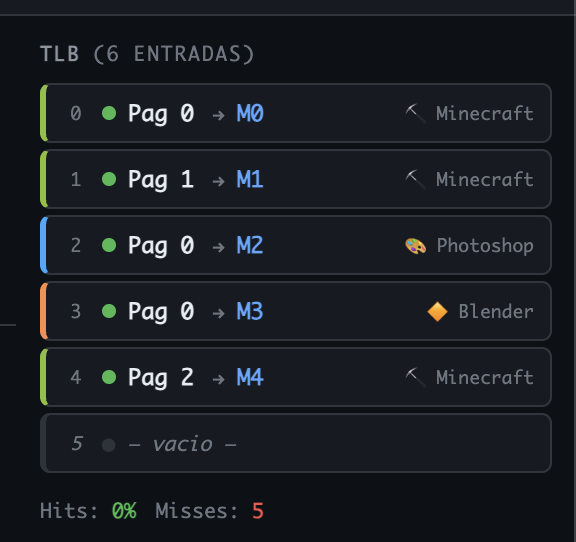
\includegraphics[width=0.85\textwidth]{captures/cap05.png}
  \caption{Panel derecho mostrando la TLB con 6 slots activos. Cada entrada está coloreada según la aplicación propietaria. Los bordes de colores permiten identificar visualmente qué app ocupa cada slot de la caché de traducciones.}
\end{figure}

\subsection{Fallo de página y algoritmo Óptimo de Belady}

Cuando una página no está en RAM (bit P=0), ocurre un \textbf{fallo de página}:

\begin{enumerate}[leftmargin=1.5cm]
  \item Se lee la página desde disco (I/O simulado con archivos binarios reales)
  \item Si hay marcos libres, se asigna uno directamente
  \item Si la RAM está llena, el \textbf{algoritmo Óptimo de Belady} selecciona la víctima:
        la página cuyo próximo uso esté \textit{más lejano en el futuro} (o que no se
        vuelva a usar)
  \item Si la víctima tiene bit D=1 (dirty), se escribe al disco antes de desalojar
  \item La nueva página se carga en el marco liberado
\end{enumerate}

El panel central muestra el \textbf{análisis del Óptimo} en tiempo real: una tabla con
la distancia al próximo uso de cada página en RAM, la víctima resaltada en rojo con
etiqueta \textit{NUNCA}, \textit{lejano} o \textit{cerca}.

\newpage

% ─── 5. INTERFAZ WEB ──────────────────────────
\section{Interfaz Web Interactiva}

\subsection{Diseño general}

La interfaz utiliza un layout de tres columnas en tema oscuro (paleta GitHub Dark):

\begin{lstlisting}[caption=Estructura de la interfaz en tres paneles]
┌──────────────┬──────────────────────────┬─────────────┐
│ Panel Izq.   │ Panel Central (scroll)   │ Panel Der.  │
│              │                          │             │
│ Procesos     │ Evento actual            │ TLB 8 slots │
│ PTBR         │ Analisis Optimo          │             │
│ Tabla pags   │ Proximas referencias     │ Historial   │
│              │ Barra RAM 8 GB           │ reciente    │
│              │ Grid de marcos fisicos   │             │
└──────────────┴──────────────────────────┴─────────────┘
└─────────── Stats: Faults | Hit Rate | I/O ────────────┘
\end{lstlisting}

\subsection{Barra de RAM gráfica}

La barra RAM representa visualmente los 8 GB del sistema. Cada marco físico ocupa
un slot proporcional coloreado por la aplicación que lo ocupa:

\begin{itemize}[leftmargin=1.5cm]
  \item Color sólido del proceso propietario
  \item Bits D/R visibles dentro del slot
  \item Marco activo con borde azul brillante
  \item Leyenda de aplicaciones con su porcentaje de RAM ocupada
  \item Escala que muestra la proporción real (ej: ``24 KB de 8 GB'')
\end{itemize}

\subsection{Grid de marcos físicos}

Tarjetas individuales por cada marco que muestran:
\begin{itemize}[leftmargin=1.5cm]
  \item Borde de 3px del color de la aplicación propietaria
  \item Identificador del marco, proceso, página y bits P/D/R
  \item Dirección física real (del buffer ctypes)
  \item Animación \texttt{anim-in} al cargar una página nueva
  \item Animación \texttt{anim-hit} en TLB hit
  \item Animación \texttt{anim-write} al escribir (bit D=1)
\end{itemize}

\begin{figure}[H]
  \centering
  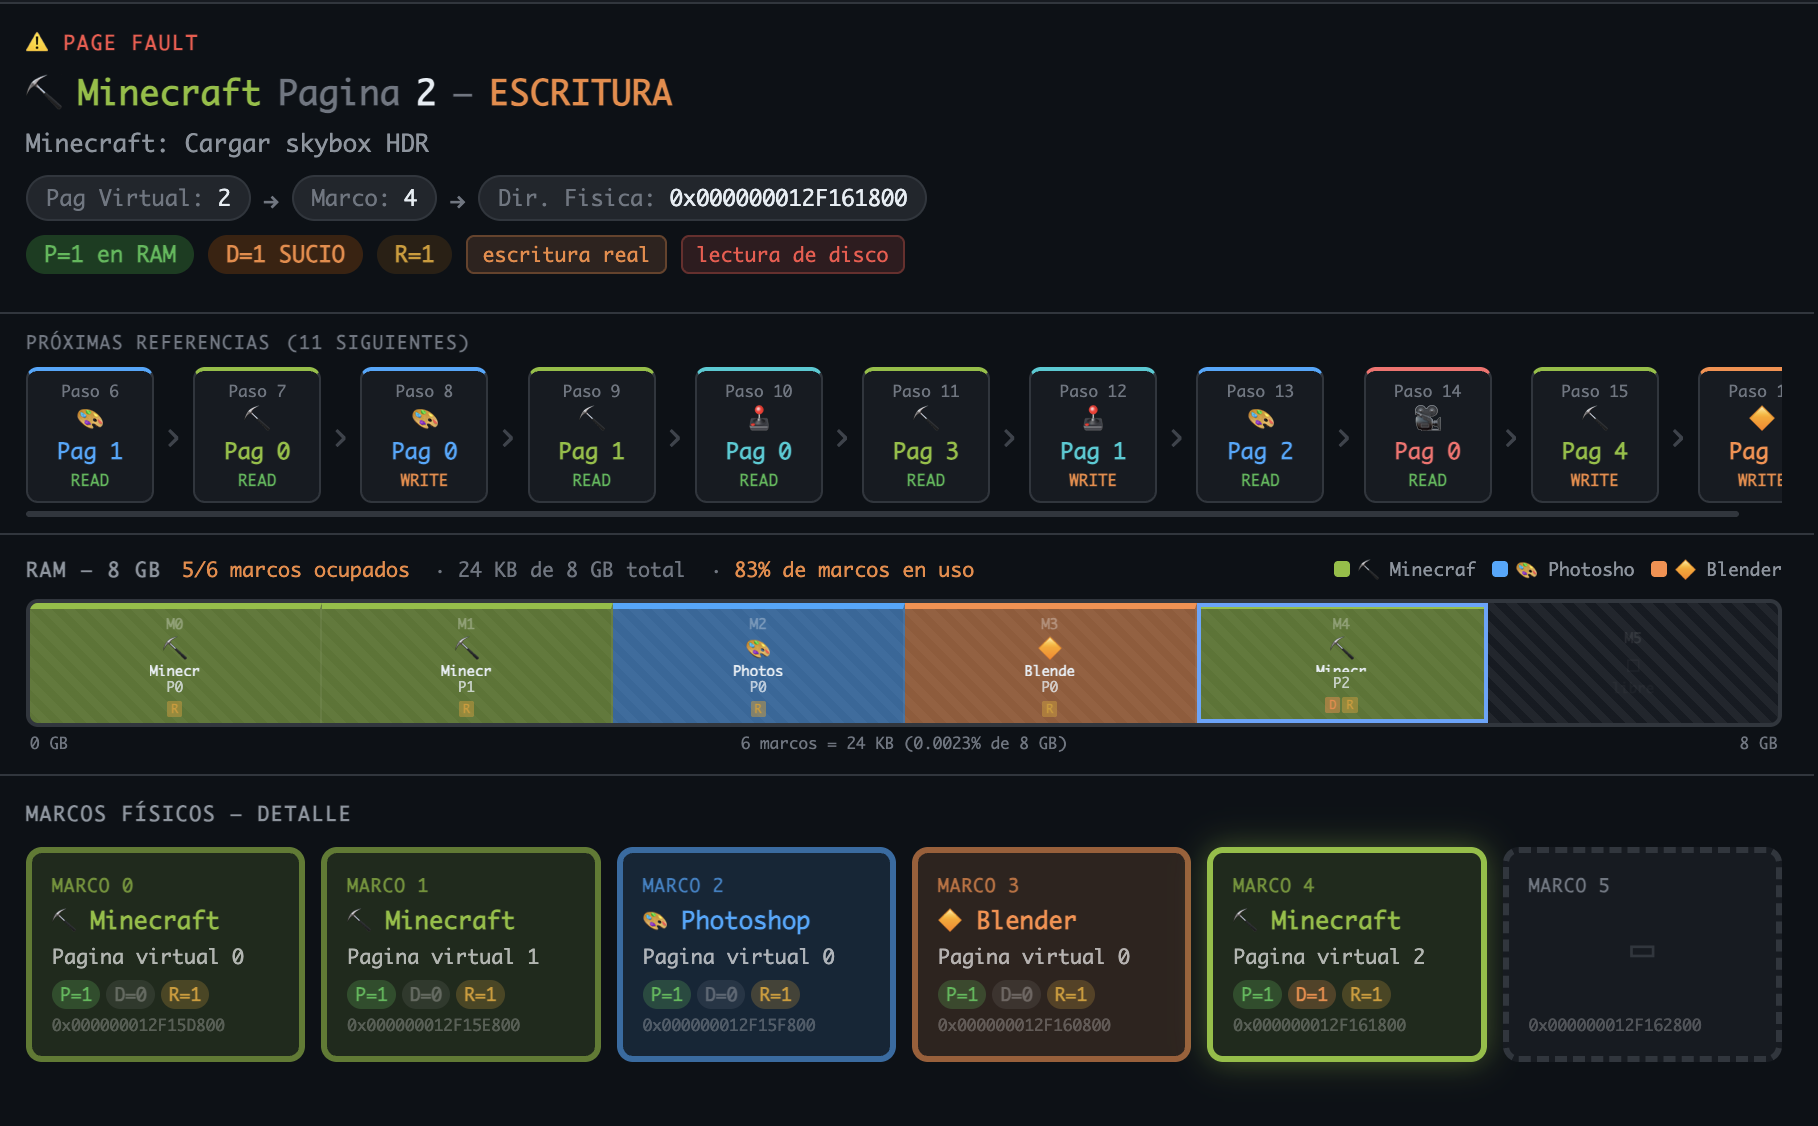
\includegraphics[width=\textwidth]{captures/cap03.png}
  \caption{Vista completa del panel central durante un PAGE FAULT. Se observa: (superior) descripción del evento con bits P/D/R y análisis del algoritmo Óptimo con la víctima seleccionada; (medio) cola de próximas 11 referencias con íconos de aplicación; (inferior) barra RAM 8 GB con slots coloreados y grid de marcos físicos con tarjetas animadas.}
\end{figure}

\subsection{Cola de próximas referencias}

Un strip horizontal scrolleable muestra las próximas 11 referencias de memoria,
permitiendo al estudiante anticipar el comportamiento del algoritmo Óptimo:

\begin{itemize}[leftmargin=1.5cm]
  \item Ícono y nombre del proceso
  \item Número de página a referenciar
  \item Tipo de operación: READ o WRITE
  \item Coloreado por aplicación
  \item La referencia actual resaltada con borde especial
\end{itemize}

\newpage

% ─── 6. CONTROLES Y NAVEGACIÓN ────────────────
\section{Controles de Navegación}

\subsection{Botones de control}

La barra de controles superior ofrece:

\begin{table}[H]
\centering
\begin{tabular}{>{\bfseries}lll}
\toprule
Control & Acción & Detalle \\
\midrule
◀ Anterior  & Retrocede un paso & Restaura snapshot completo \\
▶ Siguiente & Avanza un paso    & Guarda snapshot antes de avanzar \\
AUTO        & Ejecución automática & Velocidades: Lenta / Normal / Rápida / Turbo \\
Reiniciar   & Reinicia simulación  & Mantiene o cambia número de marcos \\
\bottomrule
\end{tabular}
\caption{Controles de navegación del simulador}
\end{table}

\subsection{Selector de marcos de RAM}

El usuario puede seleccionar el número de marcos físicos disponibles:
\textbf{3, 4, 5, 6, 8 ó 12 marcos}. Menos marcos producen más fallos de página
y son útiles para observar el algoritmo Óptimo en acción.

\subsection{Mecanismo de paso anterior (Undo)}

Antes de cada avance, el sistema guarda un snapshot completo del estado:

\begin{lstlisting}[language=python, caption=Implementación del snapshot para undo]
def _snapshot(self) -> dict:
    return {
        "paso":        self.paso,
        "stats":       dict(self.stats),
        "tlb_entradas": [
            {"pid": e.pid, "pagina": e.pagina,
             "marco": e.marco, "valida": e.valida}
            for e in self.tlb.entradas
        ],
        "tabla": {
            pid: {pg: dict(ent) for pg, ent in t.items()}
            for pid, t in self.tabla.items()
        },
        "marcos": [
            {
                "libre":   m.libre,
                "proceso": m.proceso,
                "pagina":  m.pagina,
                "bits":    dict(m.bits),
                "datos":   m.volcar() if not m.libre else None,
            }
            for m in self.marcos
        ],
        "disco_llaves": set(self.disco._archivos.keys()),
        "historial":   list(self.historial),
    }
\end{lstlisting}

El mecanismo garantiza que \textbf{todo el estado} queda capturado, incluyendo:
los buffers ctypes de 4 KB de cada marco, las entradas de la TLB, la tabla de páginas
con bits P/D/R por proceso, las estadísticas acumuladas, el historial de eventos y
los archivos de disco (swap).

\begin{figure}[H]
  \centering
  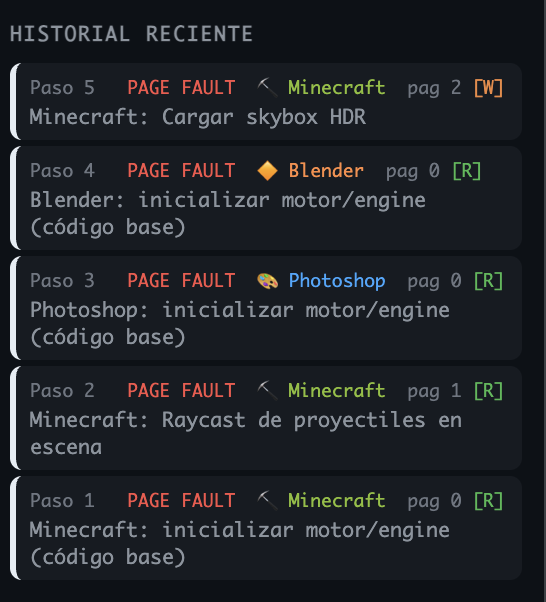
\includegraphics[width=0.85\textwidth]{captures/cap04.png}
  \caption{Historial reciente de eventos en el panel derecho. Se observa la secuencia de PAGE FAULTs de los pasos 1 al 5, con los detalles de cada acceso: proceso, página, tipo (READ/WRITE) y resultado (TLB HIT / PAGE FAULT). Este historial se restaura correctamente al retroceder pasos.}
\end{figure}

\newpage

% ─── 7. CADENA DE ACCESOS ─────────────────────
\section{Generación de la Cadena de Accesos}

La función \texttt{generar\_cadena()} crea una secuencia de 37 accesos estructurada en
7 fases que garantizan la demostración de todos los conceptos:

\begin{table}[H]
\centering
\begin{tabular}{>{\bfseries}clp{7cm}}
\toprule
Fase & Nombre & Descripción \\
\midrule
1 & Arranque inicial   & Cada proceso accede a su primera página → fallos de página iniciales \\
2 & TLB hits           & Reaccesos a páginas ya cargadas → hits en TLB garantizados \\
3 & RAM se llena       & Accesos a páginas nuevas hasta ocupar todos los marcos \\
4 & Reemplazos         & Primera presión: algoritmo Óptimo entra en acción \\
5 & Presión máxima     & Escrituras (WRITE) que activan bit D → dirty pages y escritura a disco \\
6 & Reaccesos          & Páginas referencadas nuevamente → algunos hits, algunos fallos \\
7 & Carga pesada       & Accesos intensivos de Minecraft y Photoshop que maximizan competencia \\
\bottomrule
\end{tabular}
\caption{Las 7 fases de la cadena de accesos generada}
\end{table}

\newpage

% ─── 8. VISUALIZACIONES Y ANIMACIONES ─────────
\section{Visualizaciones y Animaciones CSS}

\subsection{Tema visual}

La interfaz usa la \textbf{paleta GitHub Dark} como base:

\begin{lstlisting}[language=css, caption=Variables CSS del tema oscuro]
:root {
  --bg:       #0d1117;   /* fondo principal */
  --surface:  #161b22;   /* paneles */
  --border:   #30363d;   /* bordes */
  --text:     #c9d1d9;   /* texto principal */
  --muted:    #8b949e;   /* texto secundario */
  --accent:   #58a6ff;   /* azul acento */
  --green:    #3fb950;   /* TLB hit / activo */
  --orange:   #d29922;   /* advertencia */
  --red:      #f85149;   /* error / page fault */
}
\end{lstlisting}

\subsection{Colores de procesos}

Cada aplicación tiene un color único con contraste suficiente sobre el fondo oscuro:

\begin{table}[H]
\centering
\begin{tabular}{lll}
\toprule
\textbf{App} & \textbf{Color} & \textbf{Hex} \\
\midrule
Minecraft     & Verde musgo    & \texttt{\#8BBF2F} \\
Photoshop     & Azul Photoshop & \texttt{\#31A8FF} \\
Blender       & Naranja        & \texttt{\#F5792A} \\
Unity Editor  & Cian           & \texttt{\#00CCD4} \\
OBS Studio    & Rojo coral     & \texttt{\#FF6B6B} \\
Discord       & Morado         & \texttt{\#9B84EC} \\
\bottomrule
\end{tabular}
\caption{Colores asignados a cada proceso simulado}
\end{table}

\subsection{Animaciones implementadas}

\begin{table}[H]
\centering
\begin{tabular}{>{\ttfamily}lll}
\toprule
\textbf{Clase CSS} & \textbf{Trigger} & \textbf{Efecto} \\
\midrule
glow-hit   & TLB Hit en slot TLB      & Resplandor del color del proceso \\
slide-in   & Nueva entrada TLB        & Deslizamiento desde la izquierda \\
anim-in    & Página cargada en marco  & Fade + scale desde 0.8 a 1.0 \\
anim-hit   & TLB Hit en marco físico  & Pulso de borde verde \\
anim-write & Escritura (WRITE)        & Pulso de borde naranja (dirty) \\
\bottomrule
\end{tabular}
\caption{Animaciones CSS implementadas}
\end{table}

\subsection{Scroll del panel central}

El panel central usa \texttt{overflow-y: auto} para hacer scroll cuando el contenido
supera la altura de la pantalla, manteniendo el header y el footer siempre visibles:

\begin{lstlisting}[language=css, caption=CSS para scroll del panel central]
.center {
  flex: 1;
  overflow-y: auto;
  padding: 16px;
  display: flex;
  flex-direction: column;
  gap: 14px;
}

.ram-area {
  flex: 0 0 auto;  /* evita que se aplaste con flexbox */
}
\end{lstlisting}

\newpage

% ─── 9. DESPLIEGUE ────────────────────────────
\section{Despliegue en Producción}

\subsection{Configuración de Gunicorn}

En producción se usa Gunicorn como servidor WSGI:

\begin{lstlisting}[language=bash, caption=Comando de inicio en producción]
gunicorn --bind 0.0.0.0:5050 --workers 2 --timeout 120 mmu_gui:app
\end{lstlisting}

\subsection{Render (PaaS)}

El archivo \texttt{render.yaml} configura el despliegue automático en Render:

\begin{lstlisting}[language=yaml, caption=Configuración render.yaml]
services:
  - type: web
    name: mmu-simulator
    env: python
    buildCommand: pip install -r requirements.txt
    startCommand: >
      gunicorn --bind 0.0.0.0:$PORT
               --workers 2
               --timeout 120
               mmu_gui:app
\end{lstlisting}

\subsection{Consideraciones de producción}

\begin{itemize}[leftmargin=1.5cm]
  \item \textbf{Sesiones}: el estado del simulador se mantiene en memoria del servidor.
        Con múltiples workers, cada sesión debe usar siempre el mismo worker (sticky sessions).
  \item \textbf{psutil en servidor}: al no haber apps pesadas en el servidor, siempre se usa
        el fallback con los perfiles predefinidos.
  \item \textbf{ctypes en Linux}: los buffers de 4 KB funcionan correctamente en el entorno
        de Render (Linux x86-64).
\end{itemize}

\newpage

% ─── 10. CONCEPTOS DEMOSTRADOS ────────────────
\section{Conceptos de Sistemas Operativos Demostrados}

\begin{table}[H]
\centering
\begin{tabular}{>{\bfseries}lp{9cm}}
\toprule
Concepto & Qué se observa en la simulación \\
\midrule
Paginación           & Páginas de 4 KB cargadas en marcos físicos de RAM real \\
Tabla de páginas     & PTBR apuntando a tabla con entradas P/D/R por proceso \\
TLB                  & Caché de 8 slots: hits animados, misses que consultan tabla \\
Fallo de página      & Lectura desde disco, asignación de marco libre \\
Algoritmo Óptimo     & Análisis de uso futuro, selección de la víctima más lejana \\
Dirty page           & Bit D=1 provoca escritura a disco antes de desalojar \\
Multiprogramación    & 6 procesos compitiendo simultáneamente por la misma RAM \\
Memoria física real  & Direcciones reportadas son reales del proceso del SO \\
I/O de disco         & Archivos binarios reales simulan el swap/paginación \\
Hit rate             & Estadística en tiempo real del rendimiento de la TLB \\
\bottomrule
\end{tabular}
\caption{Conceptos de sistemas operativos demostrados por el simulador}
\end{table}

\newpage

% ─── 11. CONCLUSIONES ─────────────────────────
\section{Conclusiones}

\subsection{Resultados obtenidos}

El simulador de MMU desarrollado cumple con todos los objetivos propuestos:

\begin{enumerate}[leftmargin=1.5cm]
  \item \textbf{Realismo técnico}: el uso de \texttt{ctypes} para asignar buffers reales
        del sistema operativo hace que las direcciones físicas mostradas sean verídicas,
        no simuladas, dando al estudiante una experiencia auténtica de cómo funciona
        la gestión de memoria a nivel del hardware.

  \item \textbf{Simulación convincente}: el uso de aplicaciones reales reconocibles
        (Minecraft, Photoshop, Blender) con valores de RAM proporcionales a sus usos
        reales hace la simulación más intuitiva y memorable que los ejemplos tradicionales
        con procesos P1, P2, P3.

  \item \textbf{Visualización completa}: todas las estructuras de datos clave de una MMU
        son visibles simultáneamente — PTBR, tabla de páginas, TLB, marcos físicos, barra
        de RAM — permitiendo observar cómo interactúan en tiempo real.

  \item \textbf{Aprendizaje activo}: los controles de navegación (avanzar, retroceder,
        auto-play) permiten al estudiante examinar cada transición a su propio ritmo,
        incluyendo retroceder para re-analizar decisiones del algoritmo Óptimo.

  \item \textbf{Algoritmo Óptimo visible}: la cola de próximas referencias y la tabla
        de análisis del Óptimo hacen explícito el razonamiento del algoritmo de Belady,
        que normalmente es abstracto e invisible.
\end{enumerate}

\subsection{Posibles extensiones}

\begin{itemize}[leftmargin=1.5cm]
  \item Implementar otros algoritmos de reemplazo (LRU, Clock, FIFO) para comparación
  \item Migrar el frontend a Next.js con animaciones Framer Motion para mayor fluidez
  \item Añadir modo multisesión con sesiones Flask y base de datos para persistencia
  \item Soporte para segmentación además de paginación
  \item Exportar la simulación como video o GIF para uso en presentaciones
\end{itemize}

\newpage

% ─── REFERENCIAS ──────────────────────────────
\section*{Referencias}
\addcontentsline{toc}{section}{Referencias}

\begin{enumerate}[leftmargin=1.5cm]
  \item Silberschatz, A., Galvin, P. B., \& Gagne, G. (2018).
        \textit{Operating System Concepts} (10th ed.). Wiley.

  \item Tanenbaum, A. S., \& Bos, H. (2014).
        \textit{Modern Operating Systems} (4th ed.). Pearson.

  \item Belady, L. A. (1966). A study of replacement algorithms for a virtual-storage
        computer. \textit{IBM Systems Journal}, 5(2), 78–101.

  \item Python Software Foundation. (2024).
        \textit{ctypes — A foreign function library for Python}.
        \url{https://docs.python.org/3/library/ctypes.html}

  \item Pallets Projects. (2024). \textit{Flask Documentation}.
        \url{https://flask.palletsprojects.com/}

  \item Rodolà, G. (2024). \textit{psutil Documentation}.
        \url{https://psutil.readthedocs.io/}
\end{enumerate}

\end{document}
